\documentclass[10pt,xcolor=pdftex,dvipsnames,table]{beamer}

\usetheme{Boadilla}
%\useoutertheme[subsection=false]{smoothbars}
\usefonttheme{serif}
\usecolortheme{seagull} % dove fly seagull
\useinnertheme{rounded}
\usepackage{pifont}
\usepackage{time}       % date and time
\usepackage{url}
\usepackage{graphicx}
\usepackage[T1]{fontenc}    % european characters
% \usepackage{pgothic}
\usepackage{yfonts}
% \usepackage{courier}
\usepackage{amssymb,amsmath}  % use mathematical symbols
\usepackage{palatino}      % use palatino as the default font
\usepackage{listings}   % insert python code into presentation
\usepackage{multirow}
\usepackage{soul}   % for strikethroughs

\setbeamercovered{transparent}
\setbeamertemplate{itemize subitem}[triangle]
\setbeamertemplate{navigation symbols}{}

\newcommand{\tc}{\textcolor}
\newcommand{\select}{$\leadsto~$}
\newcommand{\fb}{\framebox}
\def\ra{$\rightarrow$\,\,}
\definecolor{cadet}{rgb}{0.33, 0.41, 0.47}
\newcommand{\hi}[1]{{\color{cadet}\textsl{#1}}}
\newcommand{\chacha}[1]{\centering{\scalebox{2}{\fontsize{12pt}{0pt}\normalfont{#1}}}}
\newcommand{\chapter}[1]{\begin{frame}{}\chacha{#1}\end{frame}}
\newcommand{\chapterDouble}[2]{\begin{frame}{}\chacha{#1}\\\medskip\chacha{#2}\end{frame}}
\newcommand{\resetEnv}{
  \colorlet{structure}{mystruct}
  \beamertemplateshadingbackground{blue!5}{gray!10}
  \beamertemplateshadingbackground{white}{white}
}
\usepackage{mathtools}
\usepackage{xcolor}
\usepackage{verbatim}
\usepackage{listings}
\usepackage{keystroke}

\definecolor{byzantium}{rgb}{0.44, 0.16, 0.39}
\definecolor{ferrariRed}{rgb}{1.0, 0.11, 0.0}
\definecolor{arsenic}{rgb}{0.23, 0.27, 0.29}

% https://transfer.sh/CR1IP/slides.pdf
% res=wgssubc-wr_cpu && acc=wgssubc-wa_cpu        # cdr[318-320,327,330-335] and gra[641-650]
% salloc --account=$acc --reservation=$res

\begin{document}

\title[Chapel workshop]{\LARGE Parallel programming in Chapel}
\author[]{{\large\sc Alex Razoumov}\\{\small alex.razoumov@westgrid.ca}\\\bigskip {\large\sc Juan
    Zuniga}\\{\small juan.zuniga@usask.ca}}
\date[June 2018]{}
\institute[]{\includegraphics[width=0.40\columnwidth]{./logos/WG-Logo-Jan16}
  \hspace{.65cm}\includegraphics[width=0.30\columnwidth]{./logos/ccLogo}}

\begin{frame}
  \titlepage
\end{frame}

\newcommand{\tnij}{\ensuremath{T^{(n)}_{i,j}}}

% language syntax and the compiler, the notions of locality and parallelism and how they are orthogonal
% concepts in Chapel

\begin{frame}{Why another language? \qquad{\large\url{http://chapel.cray.com}}}
  \begin{itemize}\setlength{\itemsep}{2mm}
  \item High-level parallel programming language
    \smallskip
    {\let\small\footnotesize \small
      \begin{itemize}\setlength{\itemsep}{0.5mm}
      \item ``Python for parallel programming''
      \item much easier to use and learn than MPI; few lines of Chapel code typically replace tens of lines
        of MPI code
      \item abstractions for data distribution/parallelism, task parallelism
      \item optimization for data-driven placement of subcomputations
      \item granular (``multi-resolution'') design: can bring closer to machine level if needed
      \item everything you can do in MPI (and OpenMP!), you should be able to do in Chapel
    \end{itemize}}
  % \item Shared- and distributed-memory parallelism built in
  \item Focus on performance
    \smallskip
    {\let\small\footnotesize \small
      \begin{itemize}\setlength{\itemsep}{0.5mm}
      \item compiled language; simple Chapel codes perform as well as optimized C/C++/Fortran code
      \item reportedly, very complex Chapel codes run at $\sim$70\% performance of a similar well-tuned
        MPI code (not bad, but room to improve)
    \end{itemize}}
  \item Perfect language for learning parallel programming for beginners
  \item Open-source: can compile on all Unix-like platforms, precompiled for MacOS (single-locale via
    Homebrew), Docker image \url{http://dockr.ly/2vJbi06} (simulates a multi-locale environment)
  \item \tc{red}{Fairly small community at the moment: too few people know/use Chapel
    ~$\Longleftrightarrow$~ too few HPC centers install and promote it}
  \end{itemize}
\end{frame}

\begin{frame}{Useful links}
  \begin{itemize}\setlength{\itemsep}{3mm}
  \item Slides from \url{https://chapel-lang.org}
    \begin{itemize}\setlength{\itemsep}{0.5mm}
    \item \href{http://chapel.cray.com/tutorials/ACCU2017/03-DataPar.pdf}{\tc{Mahogany}{\it Data
      parallelism}}
    \item \href{https://chapel-lang.org/tutorials/ACCU2017/04-TaskPar.pdf}{\tc{Mahogany}{\it Task
        parallelism}}
    \item \href{https://chapel-lang.org/tutorials/ACCU2017/05-Locality.pdf}{\tc{Mahogany}{\it
        Locality / Affinity Features}}
    \item \href{https://chapel-lang.org/tutorials/ACCU2017/06-DomainMaps.pdf}{\tc{Mahogany}{\it
        Domain Maps / Distributions}}
    \end{itemize}
  \item Watch \href{https://youtu.be/0DjIdRJIqRY}{\tc{Mahogany}{\it Chapel: Productive, Multiresolution
      Parallel Programming}} talk by Brad Chamberlain
  \item \href{http://chapel-for-python-programmers.readthedocs.io/basics.html}{\tc{Mahogany}{\it
      Getting started guide for Python programmers}}
  \item \url{https://learnxinyminutes.com/docs/chapel}
  \item Concise \href{http://faculty.knox.edu/dbunde/teaching/chapel/tutorial-1.9.html}{\tc{Mahogany}{\it
      Chapel tutorial}} by David Bunde
  \item Documentation and examples for various Chapel modules in \texttt{\$CHPL\_HOME/modules/}, e.g.,
    \texttt{standard/} or \texttt{dists/}
  \item \url{https://stackoverflow.com/questions/tagged/chapel}
  \end{itemize}
\end{frame}

\begin{frame}{Our workshop}
  \vspace{-3mm}
  \begin{columns}[]
    \column{0.30\textwidth}
    \setbeamercolor{block body}{bg=orange!10,fg=black}
    \begin{block}{}
      \begin{center}
        {\sc \underline{Part 1:} basic language features}
      \end{center}
      \vspace{-2mm}
      {\let\normalsize\footnotesize \normalsize
        \begin{itemize}\setlength{\itemsep}{0.6mm}
        \item running single-locale Chapel codes on Cedar
          {\let\small\scriptsize \small
            \begin{itemize}\setlength{\itemsep}{0.5mm}
            \item interactive jobs vs. batch jobs
          \end{itemize}}
        \item quicky on running Chapel on your laptop
        \item problem description: heat transfer equation
        \item variables
        \item ranges and arrays
        \item conditionals
        \item \tc{Mahogany}{\texttt{for}} loops
        \item config variables
        \item timing code execution
        \end{itemize}}
      \begin{center}
        \href{http://bit.ly/2CDRuxQ}{\tc{Mahogany}{\it See lesson notes}}
      \end{center}
      % \smallskip{\scriptsize \tc{RawSienna}{collaborative notes\\\vspace{-1.5mm}\url{http://bit.ly/chapelone}}}
    \end{block}
    \column{0.30\textwidth}
    \setbeamercolor{block body}{bg=orange!20,fg=black}
    \begin{block}{}
      \begin{center}
        {\sc \underline{Part 2:} Task Parallelism}
      \end{center}
      \vspace{-2mm}
      {\let\normalsize\footnotesize \normalsize
        \begin{itemize}\setlength{\itemsep}{1mm}
        \item parallel concepts
          {\let\small\scriptsize \small
            \begin{itemize}\setlength{\itemsep}{0.5mm}
            \item concurrency vs. true parallelism
            \item concurrency vs. task locality
          \end{itemize}}
        \item fire-and-forget tasks
          {\let\small\scriptsize \small
            \begin{itemize}\setlength{\itemsep}{0.5mm}
            \item \tc{Mahogany}{\texttt{begin}} statement
            \item \tc{Mahogany}{\texttt{cobegin}} statement
            \item \tc{Mahogany}{\texttt{coforall}} loops
            \item \tc{Mahogany}{\texttt{forall}} loops
          \end{itemize}}
        \item task synchronization
          {\let\small\scriptsize \small
            \begin{itemize}\setlength{\itemsep}{0.5mm}
            \item \tc{Mahogany}{\texttt{sync}} statement
            \item sync variables
            \item atomic variables
          \end{itemize}}
        \item \tc{arsenic}{task-parallelizing the heat transfer solver (if we have time)}
        \end{itemize}}
      \begin{center}
        \href{http://bit.ly/2CDHCUS}{\tc{Mahogany}{\it See lesson notes}}
      \end{center}
      % \smallskip{\scriptsize \tc{RawSienna}{collaborative
      %     notes\\\vspace{-1.5mm}\url{http://bit.ly/chapeltwo}}}
    \end{block}
    \column{0.30\textwidth}
    \setbeamercolor{block body}{bg=orange!30,fg=black}
    \begin{block}{}
      \begin{center}
        {\sc \underline{Part 3:} Domain Parallelism}
      \end{center}
      \vspace{-2mm}
      {\let\normalsize\footnotesize \normalsize
        \begin{itemize}\setlength{\itemsep}{1mm}
        \item running multi-locale Chapel codes on Cedar
        \item simple multi-locale codes
        \item domains and single-locale data parallelism
        \item distributed domains
        \item heat transfer solver on distributed domains
        \item periodic boundary conditions
        \item writing to files
        \end{itemize}}
      \begin{center}
        \href{http://bit.ly/2CC8MLW}{\tc{Mahogany}{\it See lesson notes}}
      \end{center}
      % \smallskip{\scriptsize \tc{RawSienna}{collaborative
      %     notes\\\vspace{-1.5mm}\url{http://bit.ly/chapelthree}}}
    \end{block}
  \end{columns}
\end{frame}

\begin{frame}{Numerical problem: 2D heat transfer equation}
  {\let\normalsize\small \normalsize
    \begin{itemize}\setlength{\itemsep}{2mm}
    \item Imagine a metallic plate initially at 25 degrees
    \item Simple 2D heat (diffusion) equation
      \[
        {\partial T(x,y,t)\over\partial t}={\partial^2 T\over\partial x^2}+{\partial^2 T\over\partial y^2}
        \]
      \item Discretize the solution $T(x,y,t)\approx T^{(n)}_{i,j}$ with $i=1,...,{\rm rows}$ and
        $j=1,...,{\rm cols}$
        \begin{itemize}\setlength{\itemsep}{0.5mm}
        \item {\footnotesize upper left corner is \texttt{(1,1)}, lower right corner is \texttt{(rows,cols)}}
        \end{itemize}
      \item Initial condition: \tc{Emerald}{$T^{(0)}_{i,j}=25$}
      \item Boundary condition: \quad \tc{Mahogany}{upper side $T^{(n)}_{0,1..{\rm cols}}\equiv 0$},
        \quad \tc{Mahogany}{left side $T^{(n)}_{1..{\rm rows},0}\equiv 0$}, \\ \tc{NavyBlue}{bottom side
          $T^{(n)}_{{\rm rows}+1,1..{\rm cols}} = {80\cdot j/\rm cols}$}, \quad \tc{NavyBlue}{right side
          $T^{(n)}_{1..{\rm rows},{\rm cols}+1} = 80\cdot i/{\rm rows}$}\\ \tc{NavyBlue}{(linearly
              increasing from 0 to 80 degrees)}
      \item Discretize the equation with forward Euler time stepping
        \[
          {T^{(n+1)}_{i,j}-\tnij\over\Delta t}=
          {T^{(n)}_{i+1,j}-2T^{(n)}_{i,j}+T^{(n)}_{i-1,j}\over(\Delta x)^2}+
          {T^{(n)}_{i,j+1}-2T^{(n)}_{i,j}+T^{(n)}_{i,j-1}\over(\Delta y)^2}
          \]
    \end{itemize}}
\end{frame}

\begin{frame}{Numerical problem: 2D heat transfer equation (cont.)}
  \begin{itemize}\setlength{\itemsep}{3mm}
    \item For simplicity assume $\Delta x=\Delta y=1$
    \item Use $\Delta t=1/4$
    \item The finite difference equation becomes
    \[
      T^{(n+1)}_{i,j} = {1\over4}\left[T^{(n)}_{i+1,j}+T^{(n)}_{i-1,j}+T^{(n)}_{i,j+1}+T^{(n)}_{i,j-1}\right]
    \]
    \item The objective is to find $T_{i,j}$ after a certain number of iterations, or when the system is
      in steady state
    \item Can increase the number of points in the grid to illustrate the advantage of parallelism
  \end{itemize}
\end{frame}

\begin{frame}{Serial exercise: using {\it procedures} and control flow}{Look up Chapel procedures}
  Write a Chapel code to find the root of the equation $x^5 + 8x^3 - 2x^2 + 5x - 1.2 = 0$ using the bisection
  method in the interval [-1,1]
  \begin{columns}[]
    \column{0.45\textwidth}
    \begin{itemize}\setlength{\itemsep}{3mm}
      \item Calculate the function at the ends and the midpoint of the interval
      \item Depending on the signs of the three computed values, let the midpoint be either the new left
      or the new right end
      \item Repeat until your error is below $\Delta x=10^{-8}$
    \end{itemize}
    \column{0.55\textwidth}
    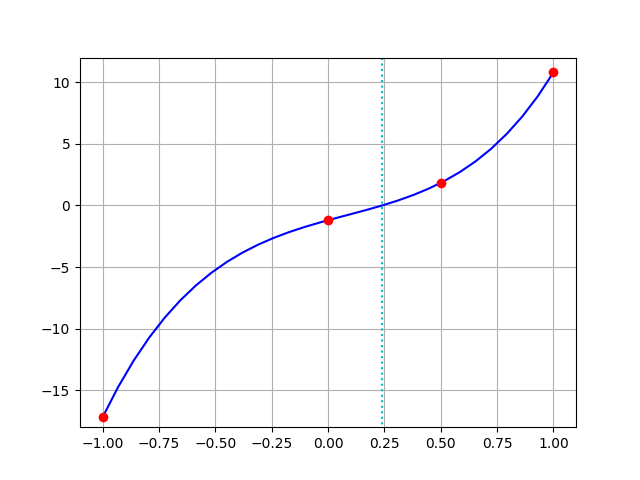
\includegraphics[width=0.95\columnwidth]{figs/bisection.png}
  \end{columns}
\end{frame}

\begin{frame}{Parallelism vs. TASK LOCALITY}
  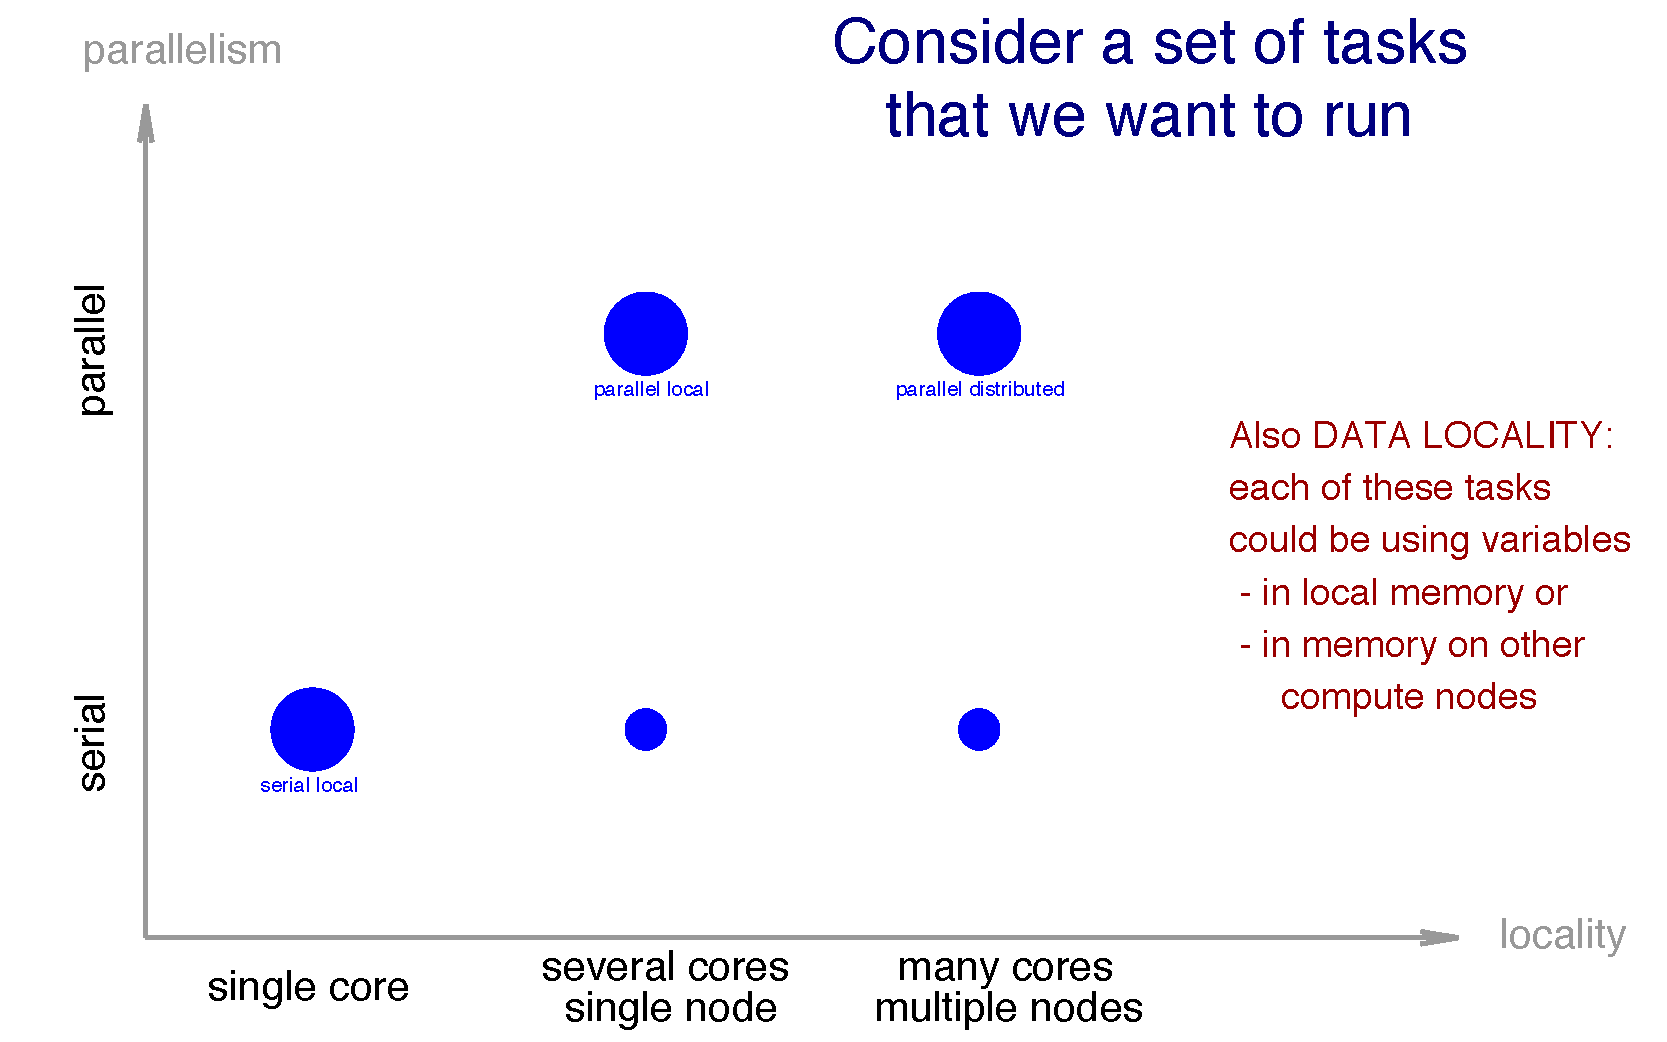
\includegraphics[width=1.0\columnwidth]{orthogonal.pdf}
\end{frame}

\begin{frame}{Task- vs. data-parallel}
  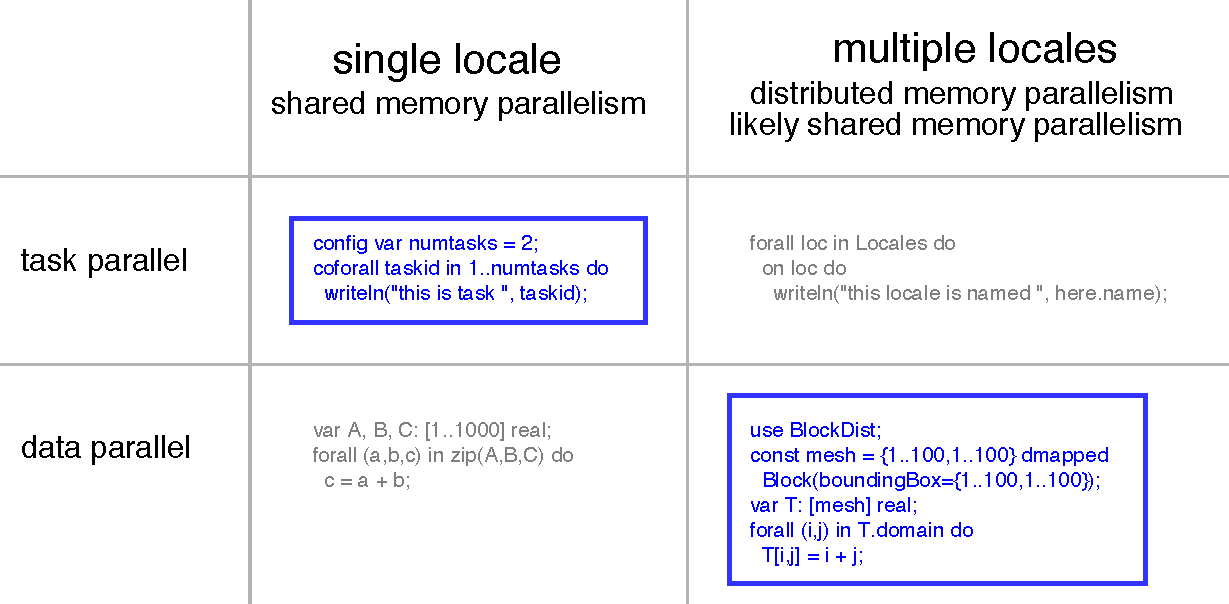
\includegraphics[width=1.0\columnwidth]{parallel.pdf}
\end{frame}

\begin{frame}{Array decomposition}
  \begin{center}
    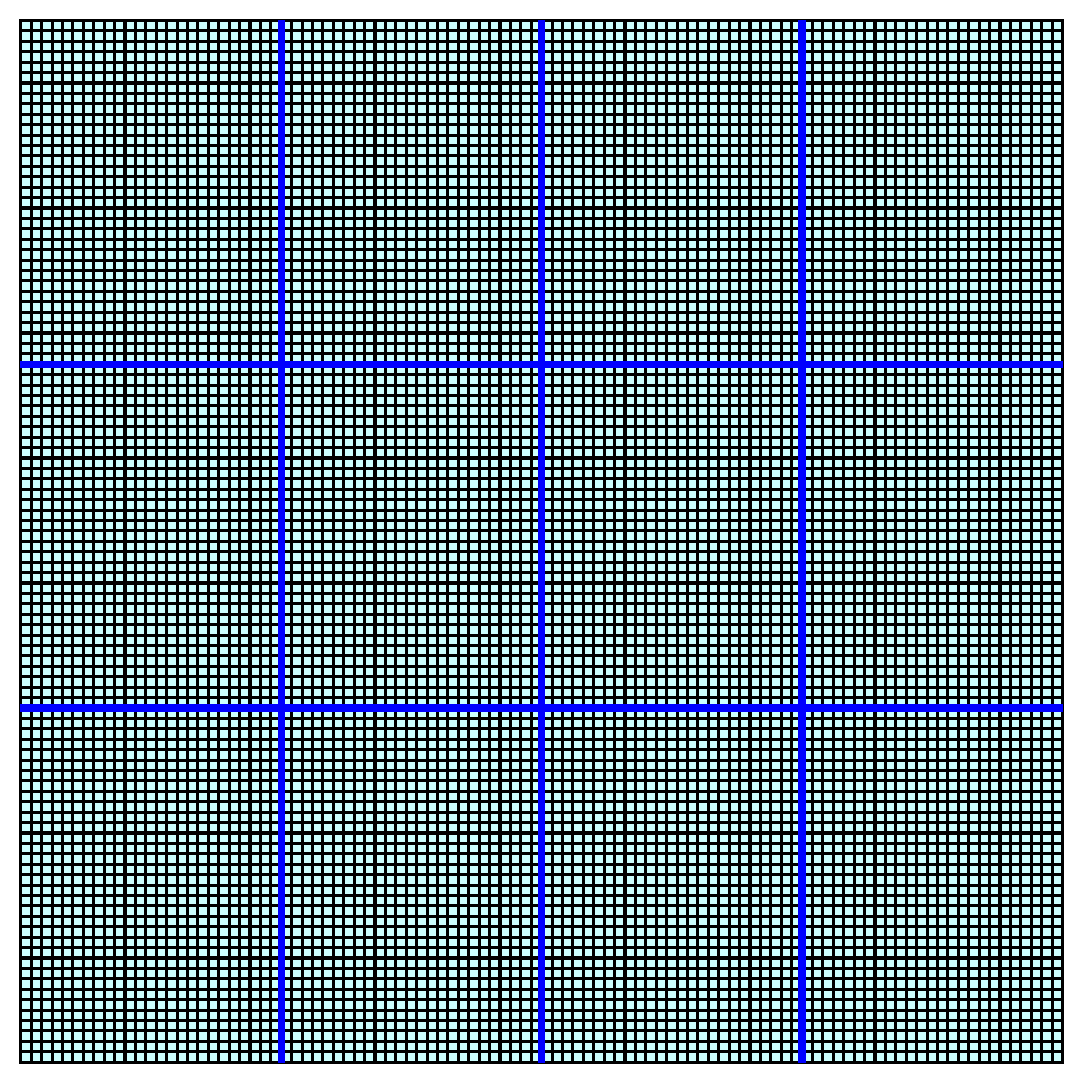
\includegraphics[width=0.68\columnwidth]{decomposition.pdf}
  \end{center}
\end{frame}

\begin{frame}{Race condition}
  \begin{center}
    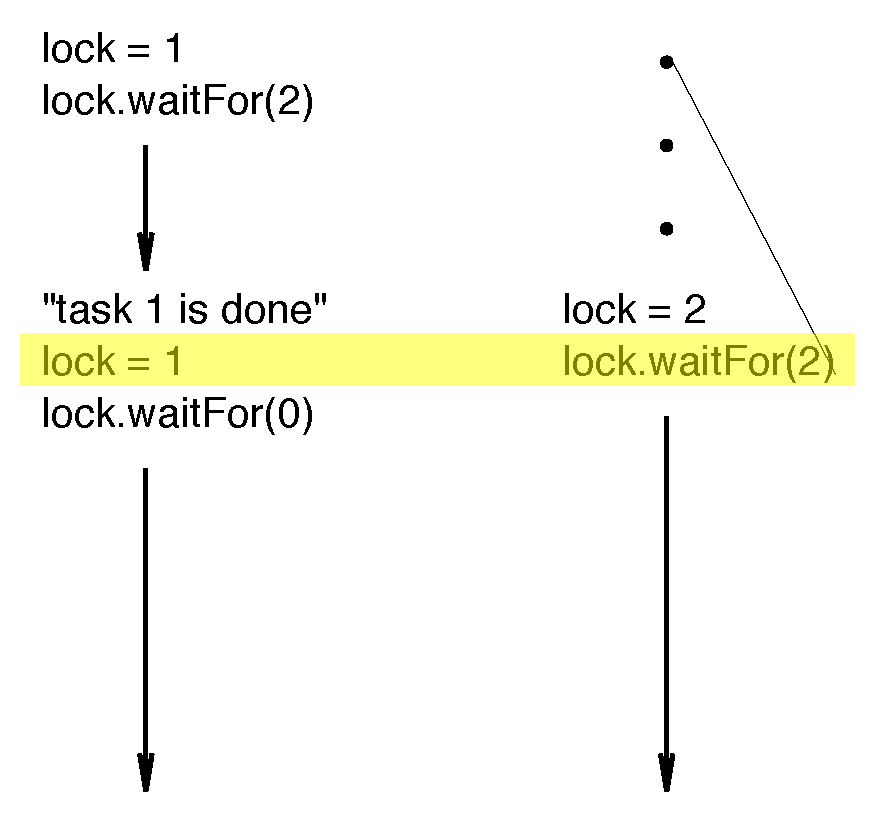
\includegraphics[width=0.65\columnwidth]{raceCondition.pdf}
  \end{center}
\end{frame}

\begin{frame}{Data-parallel exercise: compute $\pi$ with \texttt{forall} loop}
  Write a parallel Chapel code to compute $\pi$ by calculating the integral numerically through summation
  {\Large
    \[
    \pi=\int_0^1{4\,dx\over 1+x^2}
    \]}
\end{frame}

\begin{frame}{Parallelism cheatsheet}
  {\let\normalsize\footnotesize \normalsize
    \begin{itemize}\setlength{\itemsep}{0.3mm}
    \item \tc{Mahogany}{\texttt{for}} is a serial loop; \quad\tc{Mahogany}{\texttt{a..\#n}} means n
      iterations, \quad\tc{Mahogany}{\texttt{a..b}} means b-a+1 iterations
    \item \tc{Mahogany}{\texttt{forall}} loop is executed cooperatively by all local cores in parallel,
      or by remote locales that own the corresponding indices/elements (subdividing their local
      iterations among their local cores); number of threads scales to the number of available cores
    \item \tc{Mahogany}{\texttt{coforall}} loop creates a new task per each iteration (cycling through
      locales or tasks inside a locale)
    \item \tc{Mahogany}{\texttt{begin \{ ... \}}} spins statements inside off into a new task
    \item \tc{Mahogany}{\texttt{sync \{ ... \}}} pauses until the children have synced back up
    \item \tc{Mahogany}{\texttt{cobegin \{ line1 line2 line3 \}}} runs each line in a new task; can be
      grouped with \{\}
    \item Built-in variables and arrays
      {\let\small\scriptsize
        \begin{itemize}\setlength{\itemsep}{0.1mm}
        \item \tc{Mahogany}{\texttt{numLocales}} is the number of locales
        \item \tc{Mahogany}{\texttt{Locales}} stores an array of compute nodes on which the program is
          executing
        \item \tc{Mahogany}{\texttt{locale.id}} is the ID of the current locale
        \item \tc{Mahogany}{\texttt{locale.maxTaskPar}} is the runtime maximum number of tasks on the
          current local
        \item \tc{Mahogany}{\texttt{locale.numCores}} is the locale's number of compute cores
        \item \tc{Mahogany}{\texttt{locale.name}} is a locale's name
        \item \tc{Mahogany}{\texttt{here}} evaluates to the locale on which the current task is running
        \end{itemize}}
    \item Distributions
      {\let\small\scriptsize
        \begin{itemize}\setlength{\itemsep}{0.1mm}
        \item \tc{Mahogany}{\texttt{BlockDist}} partitions indices into blocks according to a boundingBox
          domain and maps each block onto a separate locale
        \item \tc{Mahogany}{\texttt{CyclicDist}} maps indices to locales in a round-robin pattern
          starting at a given index
        \item \tc{Mahogany}{\texttt{BlockCycDist}}, \tc{Mahogany}{\texttt{DimensionalDist2D}},
          \tc{Mahogany}{\texttt{PrivateDist}}, \tc{Mahogany}{\texttt{ReplicatedDist}},
          \tc{Mahogany}{\texttt{StencilDist}}, \tc{Mahogany}{\texttt{BlockCycDim}},
          \tc{Mahogany}{\texttt{BlockDim}}, \tc{Mahogany}{\texttt{ReplicatedDim}}
      \end{itemize}}
  \end{itemize}}
\end{frame}

% forall and coforall in abstract level

% revisiting the notion of locality, where in the hardware the tasks (or the different locales) are
% running, parallel data structures, domain maps

\begin{frame}{Distributed domains}
  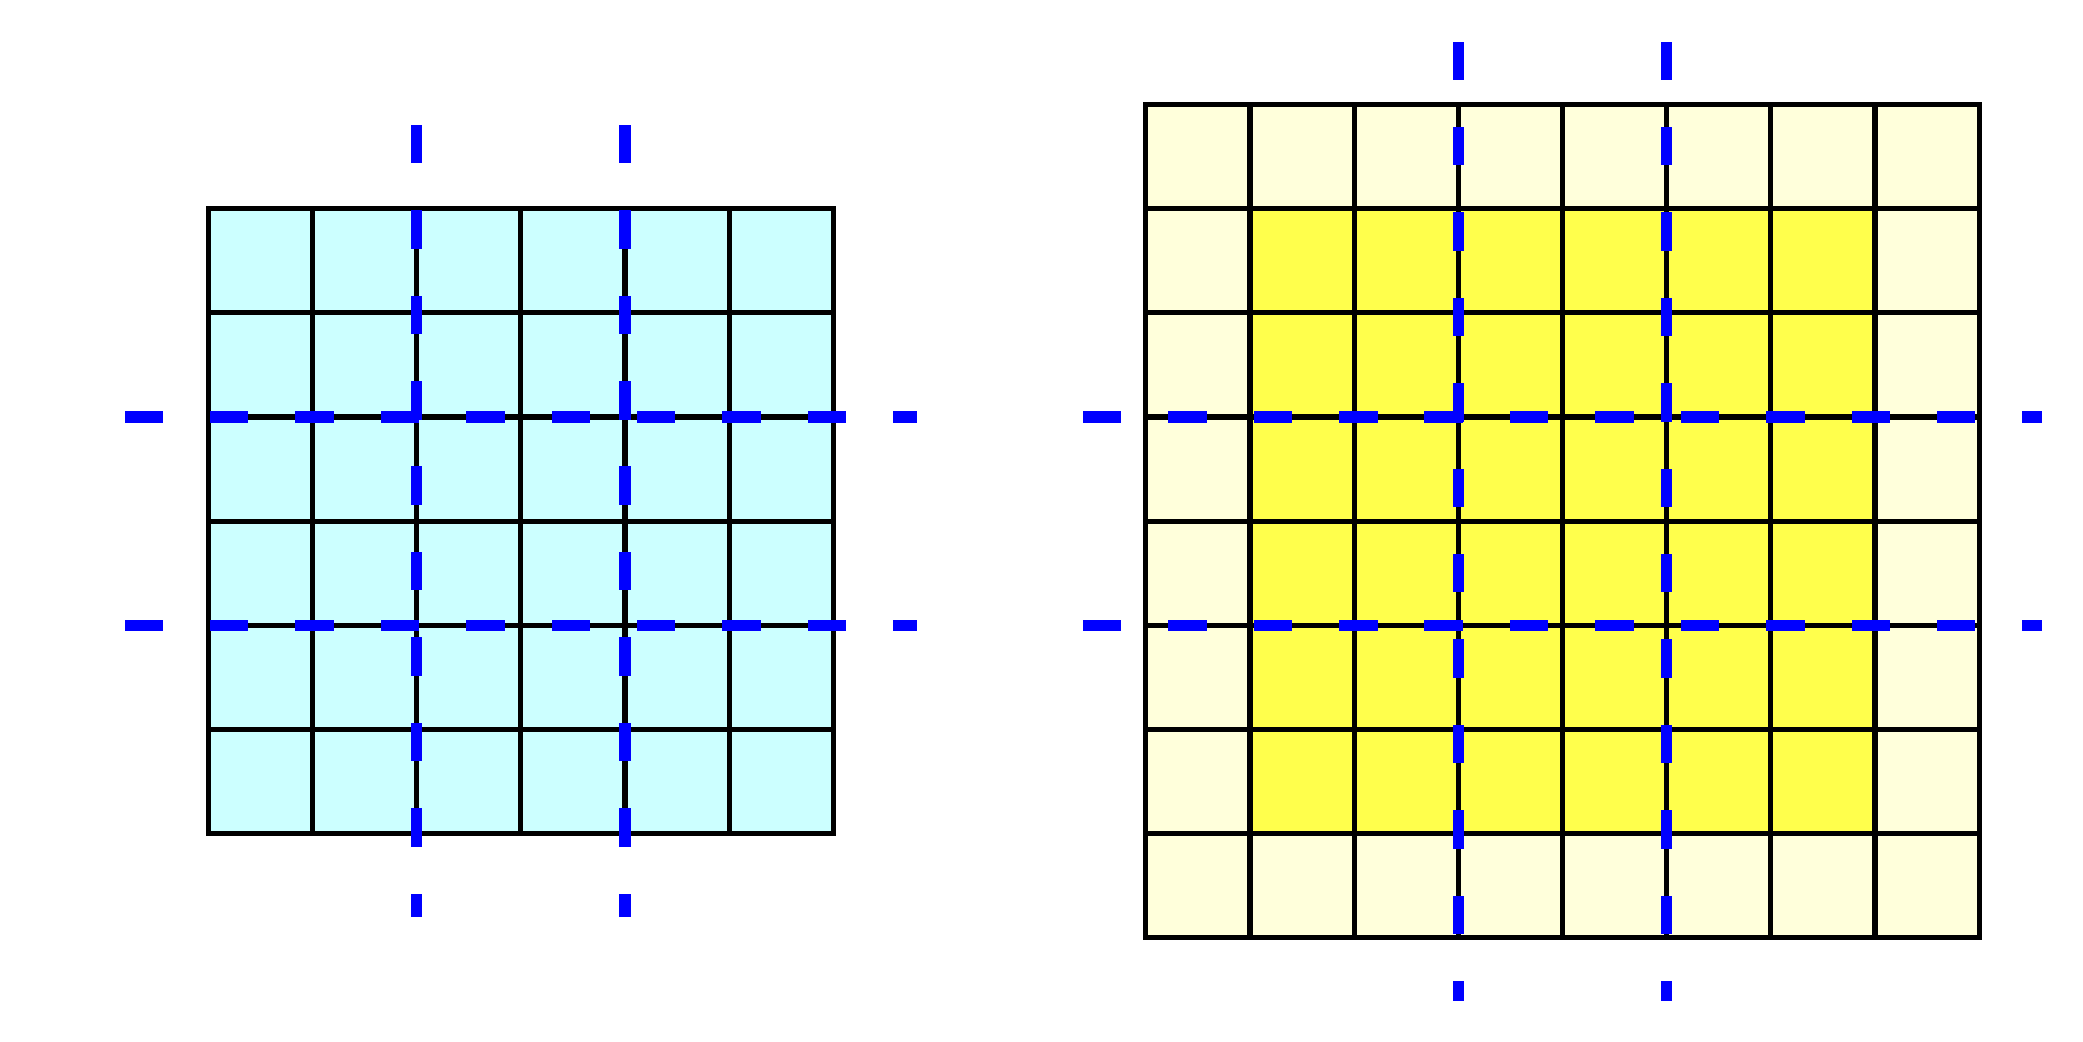
\includegraphics[width=1.0\columnwidth]{domains.pdf}
  % domain types \url{http://chapel.cray.com/tutorials/ACCU2017/03-DataPar.pdf}
\end{frame}

% http://chapel.cray.com/docs/1.14/primers/primers/distributions.html
% http://chapel.cray.com/tutorials/ACCU2017/03-DataPar.pdf
% builtin Locales variable
% - for loc in Locales {} followed by on loc {}
% - do something on Locales[1]
% become very proficient with regular domains
% blocks.chpl
% - introduce a block-distributed domain and an array of to of it
% cyclic.chpl
% evolution.chpl
% periodic.chpl
% - exercise: modify evolution.chpl to put in periodic BCs
% - check energy conservation
% - write out each timestep to an ASCII file

% iterators, I/O files, modules and other packages?
% how to call C/C++/Fortran functions from Chapel, especially popular numerical libraries

\end{document}
